% !Mode:: "TeX:UTF-8"	% read in as utf8 file.

\chapter{Basic geometries}

\section{Triangle Surface Area}
If your \num{3} points are $ \vec{A}, \vec{B}, \vec{C} $ then you may use directly (half) cross-product formula:
\begin{align}
\vec{u} &= \vec{AB} \\
\vec{v} &= \vec{AC} \\
S &= \dfrac{|\vec{u} \times \vec{v}|}{2} = \dfrac{|\vec{u}||\vec{v}||sin(\theta)|}{2}
\end{align}

that is (see the Wikipedia link to get the cross-product in $ \mathbb{R}^3 $):
\begin{equation*}
S = \dfrac{1}{2} \sqrt{(v_1 w_2 - w_1 v_2)^2 + (w_1 u_2 - u_1 w_2)^2 + (u_1 v_2 - v_1 u_2)^2}
\end{equation*}

\section{Superellipse}
\begin{figure}[!h]
	\centering
	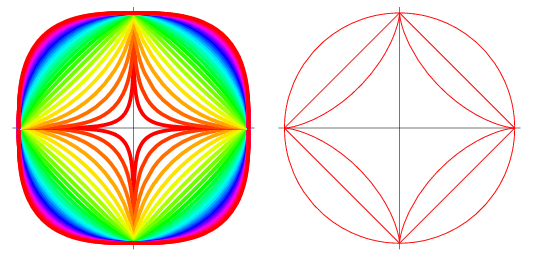
\includegraphics[width=0.7\linewidth]{Figures/Superellipses_1001}
	\caption{}
	\label{fig:superellipses1001}
\end{figure}

A superellipse is a curve with Cartesian equation

\begin{equation}
\left( \dfrac{x}{a} \right) ^ r + \left( \dfrac{y}{b} \right) ^ r = 1,
\end{equation}

first discussed in 1818 by Lamé. A superellipse may be described parametrically by

\begin{align*}
x &= a \cos ^ {\frac{2}{r}} t \\
y &= b \sin ^ {\frac{2}{r}} t \\
\end{align*}

The restriction to $ r>2 $ is sometimes made.

Superellipses with $ a=b $ are also know Lam\`{e} curve or Lam\`{e} ovals, and the case $ a=b $ with $ r=4 $ is sometimes known as the squircle. By analogy, the superellipse with $ a!=b $ and $ r=4 $ might be termed the rectellipse.

A range of superellipses are shown above, with special cases $ r=2/3 $, 1, and 2 illustrated right above. The following table summarizes a few special cases. Piet Hein used r=5/2 with a number of different a/b ratios for various of his projects. For example, he used $ a/b=6/5 $ for Sergels Torg (Sergel's Square) in Stockholm, Sweden (Vestergaard), and $ a/b=3/2 $ for his table.

\begin{table}[!h]
	\centering
	\begin{tabular}{|c|c|}
		\hline 
		$ r $ & curve \\ 
		\hline 
		$ \dfrac{2}{3} $ & (squashed) astroid \\ 
		\hline 
		1 & (squashed) diamond \\ 
		\hline 
		2 & 	ellipse \\ 
		\hline 
		$ \dfrac{5}{2} $ & Piet Hein's "superellipse" \\ 
		\hline 
		4 & rectellipse \\ 
		\hline 
	\end{tabular} 
\end{table}

If $ r $ is a rational, then a superellipse is algebraic. However, for irrational $ r $, it is transcendental. For even integers $ r=n $, the curve becomes closer to a rectangle as $ n $ increases.

The area of a superellipse is given by

\begin{equation}
\frac{4^{1-\frac{1}{r}} a b \sqrt{\pi } \text{Gamma}\left[1+\frac{1}{r}\right]}{\text{Gamma}\left[\frac{1}{2}+\frac{1}{r}\right]}
\end{equation}

\begin{figure}[h!]
	\centering
	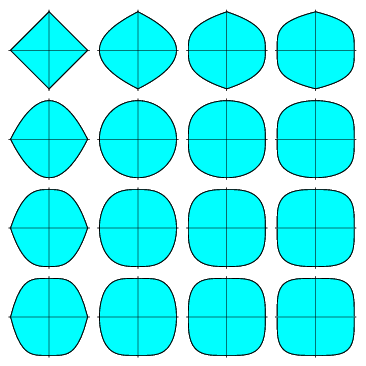
\includegraphics[width=0.7\linewidth]{Figures/SuperellipseRegions_1000}
	\caption{}
	\label{fig:superellipseregions1000}
\end{figure}


\section{Frustum volume}
If the shape parameters at left side (square) of ribs is $ b1, h1 $, at right side (square) of rib is $ b2, h2 $, then the volume of the frustum is:
\begin{equation}\label{eq: frustum volume}
\begin{split}
\mathrm{vol} &= \frac{S_1 + S_2 + \sqrt{(S_1 S_2)}}{3} l \\
&= \frac{b_1 h_1 + b_2 h_2 + \sqrt{(b_1 b_2 h_1 h_2 )}}{3} l
\end{split}
\end{equation}

the gradient of the volume is:
\begin{equation}\label{key}
\begin{split}
\frac{\partial \mathrm{vol}}{\partial b_1} & = \frac{h_1}{6} l + \frac{1}{2} \sqrt{ \frac{h_1 b_2 h_2}{b_1}} l \\
\frac{\partial \mathrm{vol}}{\partial h_1} & = \frac{b_1}{6} l + \frac{1}{2} \sqrt{ \frac{b_1 b_2 h_2}{h_1}} l \\
\frac{\partial \mathrm{vol}}{\partial b_2} & = \frac{h_2}{6} l + \frac{1}{2} \sqrt{ \frac{b_1 h_1 h_2}{b_2}} l \\
\frac{\partial \mathrm{vol}}{\partial h_2} & = \frac{b_2}{6} l + \frac{1}{2} \sqrt{ \frac{b_1 b_2 h_1}{h_2}}  l
\end{split}
\end{equation}

\section{Combined H beam volume}
let shape parameters at left side (square) of ribs is $ b_{1i}, h_{1i}, b_{2i}, h_{2i} $, at right side (square) of rib is $ b_{1j}, h_{1j}, b_{2j}, h_{2j} $, then the volume of the frustum is:
\begin{equation}\label{eq: frustum volume}
\begin{split}
\mathrm{vol} &= \frac{S_1 + S_2 + \sqrt{(S_1 S_2)}}{3} l \\
&= \frac{b_{1i} h_{1i} + b_{1j} h_{1j} + \sqrt{(b_{1i} b_{1j} h_{1i} h_{1j} )}}{3} l + \frac{b_{2i} (h_{2i} - h_{1i}) + b_{2j} (h_{2j} - h_{1j}) + \sqrt{(b_{2i} b_{2j} (h_{2i} - h_{1i}) (h_{2j} - h_{1j}) )}}{3} l 
\end{split}
\end{equation}

\section{Area and second moments of any polygon}
\begin{figure}[h!]
	\centering
	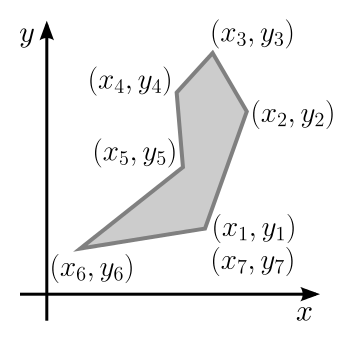
\includegraphics[width=0.4\linewidth]{Figures/Moment_of_area_of_a_polygon}
	\caption{Numbering of a polygon}
	\label{fig:numberingofapolygon}
\end{figure}

The second moment of area for any simple polygon on the XY-plane can be computed in general by summing contributions from each segment of the polygon. A polygon is assumed to have $ n $ vertices, numbered in counter-clockwise fashion. If polygon vertices are numbered clockwise, returned values will be negative, but absolute values will be correct.

\begin{align*}
A &= \frac{1}{2} \sum_{i=1}^{n} (x_i y_{i+1} - x_{i+1} y_i) \\
I_{x} &= {\frac {1}{12}}\sum_{i=1}^{n}(y_{i}^{2}+y_{i}y_{i+1}+y_{i+1}^{2})(x_{i}y_{i+1}-x_{i+1}y_{i}) \\
I_{y} &= {\frac {1}{12}}\sum _{i=1}^{n}(x_{i}^{2}+x_{i}x_{i+1}+x_{i+1}^{2})(x_{i}y_{i+1}-x_{i+1}y_{i})
\end{align*}

where  $ x_{i},y_{i} $ are the coordinates of the $ i $-th polygon vertex, for $ 1\leq i\leq n $. Also, $ x_{n+1},y_{n+1} $ are assumed to be equal to the coordinates of the first vertex, i.e., $ x_{n+1}=x_{1} $ and $ y_{n+1}=y_{1} $.

\subsection{equations for a triangle}
\begin{figure}[h!]
\centering
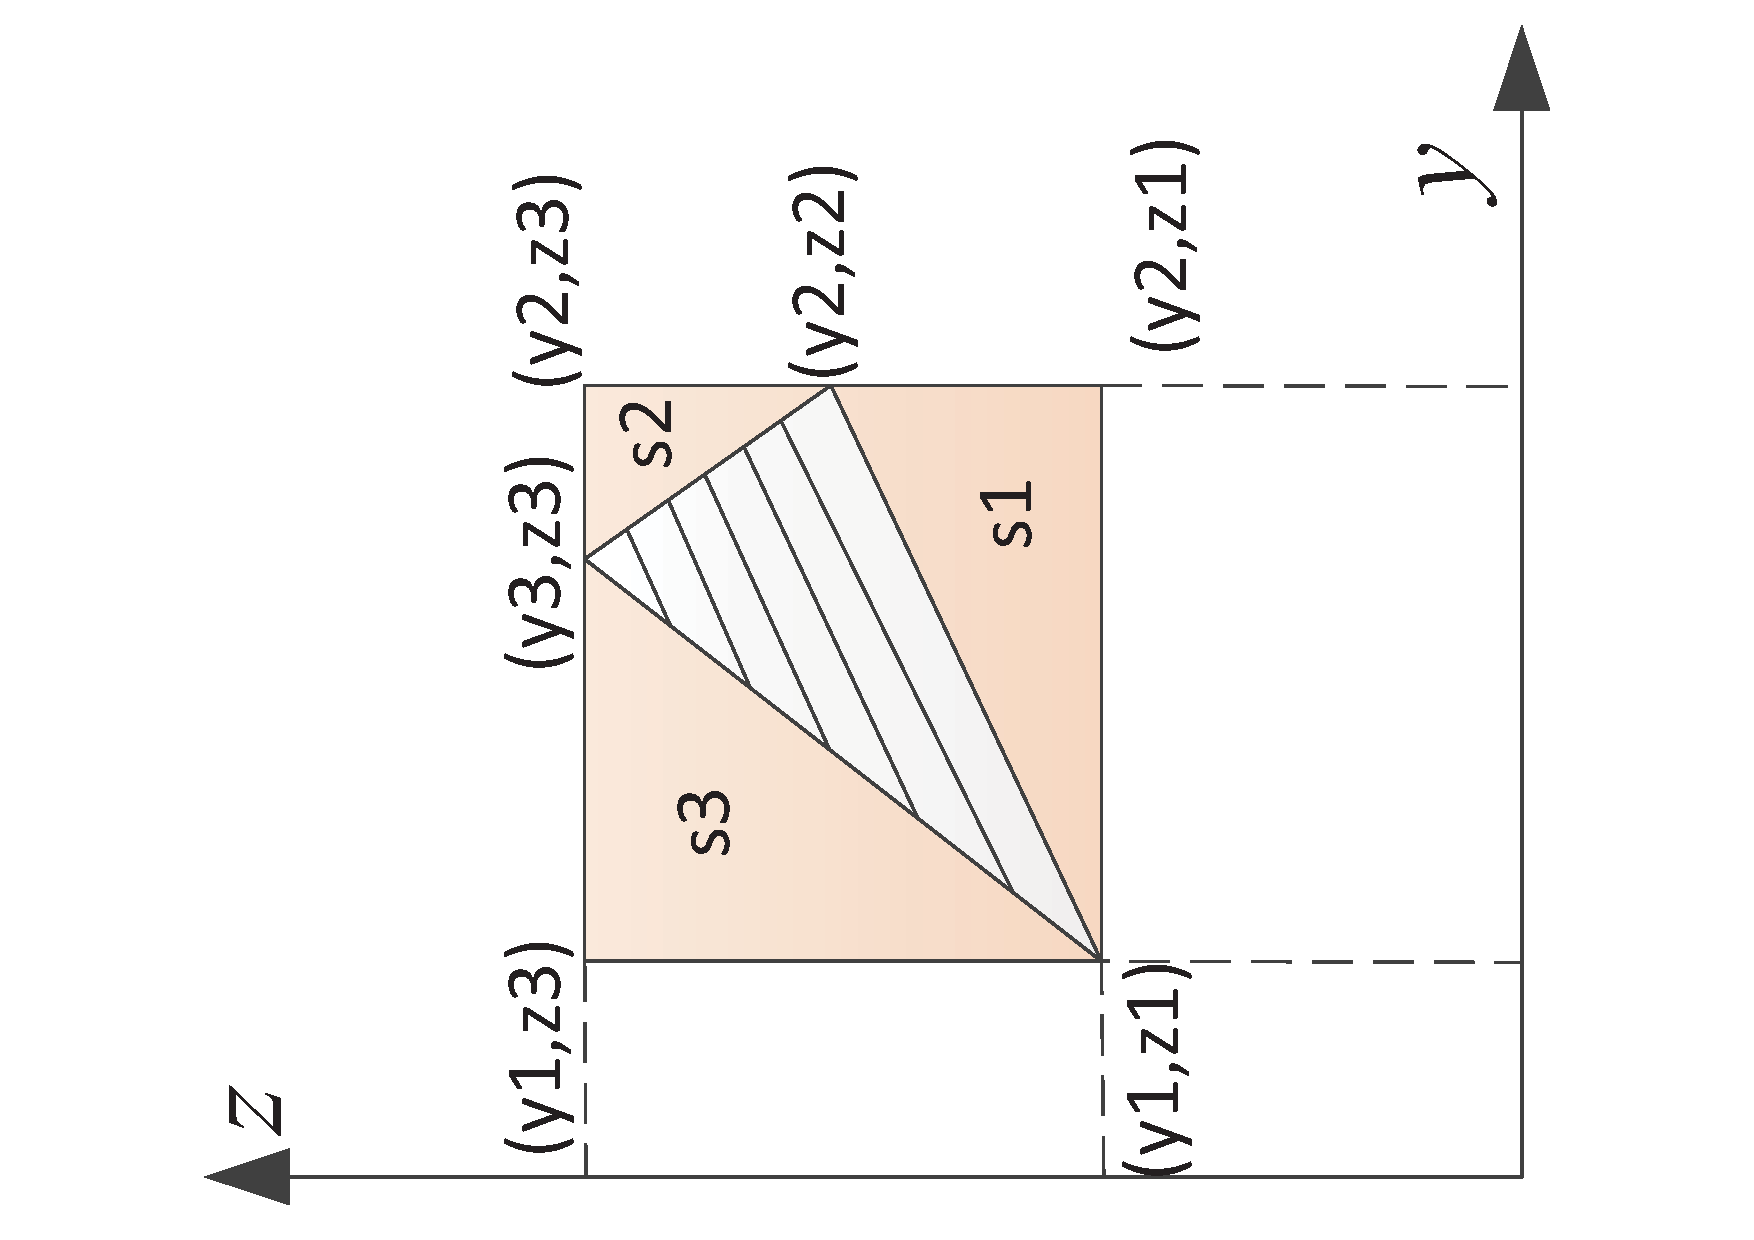
\includegraphics[width=0.7\linewidth, angle=-90]{Figures/areaMomentsForTriangle}
\caption{}
\label{fig:areamomentsfortriangle}
\end{figure}

\begin{align*}
\delta_{y_1} &= (y_2-y_1)- \frac{y_2-y_1}{z_2-z_1} (z-z_1) & \delta_{y_2} &= \frac{y_2-y_3}{z_3-z_2} (z-z_2) & \delta_{y_3} &= \frac{y_3-y_1}{z_3-z_1} (z-z_1) \\
\delta_{z_1} &= \frac{z_2-z_1}{y_2-y_1} (y-y_1 ) & \delta_{z_2 } &= \frac{z_3-z_2}{y_2-y_3} (y-y_3) & \delta_{z_3} &= (z_3-z_1)- \frac{z_3-z_1}{y_3-y_1} (y-y_1) \\
A_1 &= \int_{z_1}^{z_2} \delta_{y_1} dz & A_2 &= \int_{z_2}^{z_3} \delta_{y_2} dz & A_3 &= \int_{z_1}^{z_3} \delta_{y_3} dz \\
I_{y_1} &=\int_{z_1}^{z_2} \delta_{y_1} z^2 dz & I_{y_2 } &= \int_{z_2}^{z_3} \delta_{y_2} z^2 dz & I_{y_3} &= \int_{z_1}^{z_3} \delta_{y_3} z^2 dz \\
I_{z_1} &= \int_{y_1}^{y_2} \delta_{z_1} y^2 dz & I_{z_2 } &= \int_{y_3}^{y_2} \delta_{z_2} y^2 dz & I_{z_3} &= \int_{y_1}^{y_3} \delta_{z_3} y^2 dz
\end{align*}

\begin{align*}
A &= (y_2-y_1)(z_3-z_1)-A_1-A_2-A_3 \\
I_y &= \int_{z_1}^{z_3}(y_2-y_1) z^2 dz - I_{y_1} - I_{y_2} - I_{y_3} \\
I_z &= \int_{y_1}^{y_3}(z_3-z_1) y^2 dz - I_{z_1} - I_{z_2} - I_{z_3}
\end{align*}

The results obtained by this exact equations is euqal to the results from above section. see example in \textcolor{red}{Run\_anyPolygon.m}
